% Options for packages loaded elsewhere
\PassOptionsToPackage{unicode}{hyperref}
\PassOptionsToPackage{hyphens}{url}
\documentclass[
]{article}
\usepackage{xcolor}
\usepackage[margin=1in]{geometry}
\usepackage{amsmath,amssymb}
\setcounter{secnumdepth}{5}
\usepackage{iftex}
\ifPDFTeX
  \usepackage[T1]{fontenc}
  \usepackage[utf8]{inputenc}
  \usepackage{textcomp} % provide euro and other symbols
\else % if luatex or xetex
  \usepackage{unicode-math} % this also loads fontspec
  \defaultfontfeatures{Scale=MatchLowercase}
  \defaultfontfeatures[\rmfamily]{Ligatures=TeX,Scale=1}
\fi
\usepackage{lmodern}
\ifPDFTeX\else
  % xetex/luatex font selection
\fi
% Use upquote if available, for straight quotes in verbatim environments
\IfFileExists{upquote.sty}{\usepackage{upquote}}{}
\IfFileExists{microtype.sty}{% use microtype if available
  \usepackage[]{microtype}
  \UseMicrotypeSet[protrusion]{basicmath} % disable protrusion for tt fonts
}{}
\makeatletter
\@ifundefined{KOMAClassName}{% if non-KOMA class
  \IfFileExists{parskip.sty}{%
    \usepackage{parskip}
  }{% else
    \setlength{\parindent}{0pt}
    \setlength{\parskip}{6pt plus 2pt minus 1pt}}
}{% if KOMA class
  \KOMAoptions{parskip=half}}
\makeatother
\usepackage{color}
\usepackage{fancyvrb}
\newcommand{\VerbBar}{|}
\newcommand{\VERB}{\Verb[commandchars=\\\{\}]}
\DefineVerbatimEnvironment{Highlighting}{Verbatim}{commandchars=\\\{\}}
% Add ',fontsize=\small' for more characters per line
\usepackage{framed}
\definecolor{shadecolor}{RGB}{248,248,248}
\newenvironment{Shaded}{\begin{snugshade}}{\end{snugshade}}
\newcommand{\AlertTok}[1]{\textcolor[rgb]{0.94,0.16,0.16}{#1}}
\newcommand{\AnnotationTok}[1]{\textcolor[rgb]{0.56,0.35,0.01}{\textbf{\textit{#1}}}}
\newcommand{\AttributeTok}[1]{\textcolor[rgb]{0.13,0.29,0.53}{#1}}
\newcommand{\BaseNTok}[1]{\textcolor[rgb]{0.00,0.00,0.81}{#1}}
\newcommand{\BuiltInTok}[1]{#1}
\newcommand{\CharTok}[1]{\textcolor[rgb]{0.31,0.60,0.02}{#1}}
\newcommand{\CommentTok}[1]{\textcolor[rgb]{0.56,0.35,0.01}{\textit{#1}}}
\newcommand{\CommentVarTok}[1]{\textcolor[rgb]{0.56,0.35,0.01}{\textbf{\textit{#1}}}}
\newcommand{\ConstantTok}[1]{\textcolor[rgb]{0.56,0.35,0.01}{#1}}
\newcommand{\ControlFlowTok}[1]{\textcolor[rgb]{0.13,0.29,0.53}{\textbf{#1}}}
\newcommand{\DataTypeTok}[1]{\textcolor[rgb]{0.13,0.29,0.53}{#1}}
\newcommand{\DecValTok}[1]{\textcolor[rgb]{0.00,0.00,0.81}{#1}}
\newcommand{\DocumentationTok}[1]{\textcolor[rgb]{0.56,0.35,0.01}{\textbf{\textit{#1}}}}
\newcommand{\ErrorTok}[1]{\textcolor[rgb]{0.64,0.00,0.00}{\textbf{#1}}}
\newcommand{\ExtensionTok}[1]{#1}
\newcommand{\FloatTok}[1]{\textcolor[rgb]{0.00,0.00,0.81}{#1}}
\newcommand{\FunctionTok}[1]{\textcolor[rgb]{0.13,0.29,0.53}{\textbf{#1}}}
\newcommand{\ImportTok}[1]{#1}
\newcommand{\InformationTok}[1]{\textcolor[rgb]{0.56,0.35,0.01}{\textbf{\textit{#1}}}}
\newcommand{\KeywordTok}[1]{\textcolor[rgb]{0.13,0.29,0.53}{\textbf{#1}}}
\newcommand{\NormalTok}[1]{#1}
\newcommand{\OperatorTok}[1]{\textcolor[rgb]{0.81,0.36,0.00}{\textbf{#1}}}
\newcommand{\OtherTok}[1]{\textcolor[rgb]{0.56,0.35,0.01}{#1}}
\newcommand{\PreprocessorTok}[1]{\textcolor[rgb]{0.56,0.35,0.01}{\textit{#1}}}
\newcommand{\RegionMarkerTok}[1]{#1}
\newcommand{\SpecialCharTok}[1]{\textcolor[rgb]{0.81,0.36,0.00}{\textbf{#1}}}
\newcommand{\SpecialStringTok}[1]{\textcolor[rgb]{0.31,0.60,0.02}{#1}}
\newcommand{\StringTok}[1]{\textcolor[rgb]{0.31,0.60,0.02}{#1}}
\newcommand{\VariableTok}[1]{\textcolor[rgb]{0.00,0.00,0.00}{#1}}
\newcommand{\VerbatimStringTok}[1]{\textcolor[rgb]{0.31,0.60,0.02}{#1}}
\newcommand{\WarningTok}[1]{\textcolor[rgb]{0.56,0.35,0.01}{\textbf{\textit{#1}}}}
\usepackage{graphicx}
\makeatletter
\newsavebox\pandoc@box
\newcommand*\pandocbounded[1]{% scales image to fit in text height/width
  \sbox\pandoc@box{#1}%
  \Gscale@div\@tempa{\textheight}{\dimexpr\ht\pandoc@box+\dp\pandoc@box\relax}%
  \Gscale@div\@tempb{\linewidth}{\wd\pandoc@box}%
  \ifdim\@tempb\p@<\@tempa\p@\let\@tempa\@tempb\fi% select the smaller of both
  \ifdim\@tempa\p@<\p@\scalebox{\@tempa}{\usebox\pandoc@box}%
  \else\usebox{\pandoc@box}%
  \fi%
}
% Set default figure placement to htbp
\def\fps@figure{htbp}
\makeatother
\setlength{\emergencystretch}{3em} % prevent overfull lines
\providecommand{\tightlist}{%
  \setlength{\itemsep}{0pt}\setlength{\parskip}{0pt}}
\usepackage[]{natbib}
\bibliographystyle{plainnat}
\usepackage{bookmark}
\IfFileExists{xurl.sty}{\usepackage{xurl}}{} % add URL line breaks if available
\urlstyle{same}
\hypersetup{
  pdftitle={HW 01 - Pet names},
  pdfauthor={Tina Huynh},
  hidelinks,
  pdfcreator={LaTeX via pandoc}}

\title{HW 01 - Pet names}
\usepackage{etoolbox}
\makeatletter
\providecommand{\subtitle}[1]{% add subtitle to \maketitle
  \apptocmd{\@title}{\par {\large #1 \par}}{}{}
}
\makeatother
\subtitle{Meet the toolkit}
\author{Tina Huynh}
\date{}

\begin{document}
\maketitle

{
\setcounter{tocdepth}{2}
\tableofcontents
}
\begin{figure}
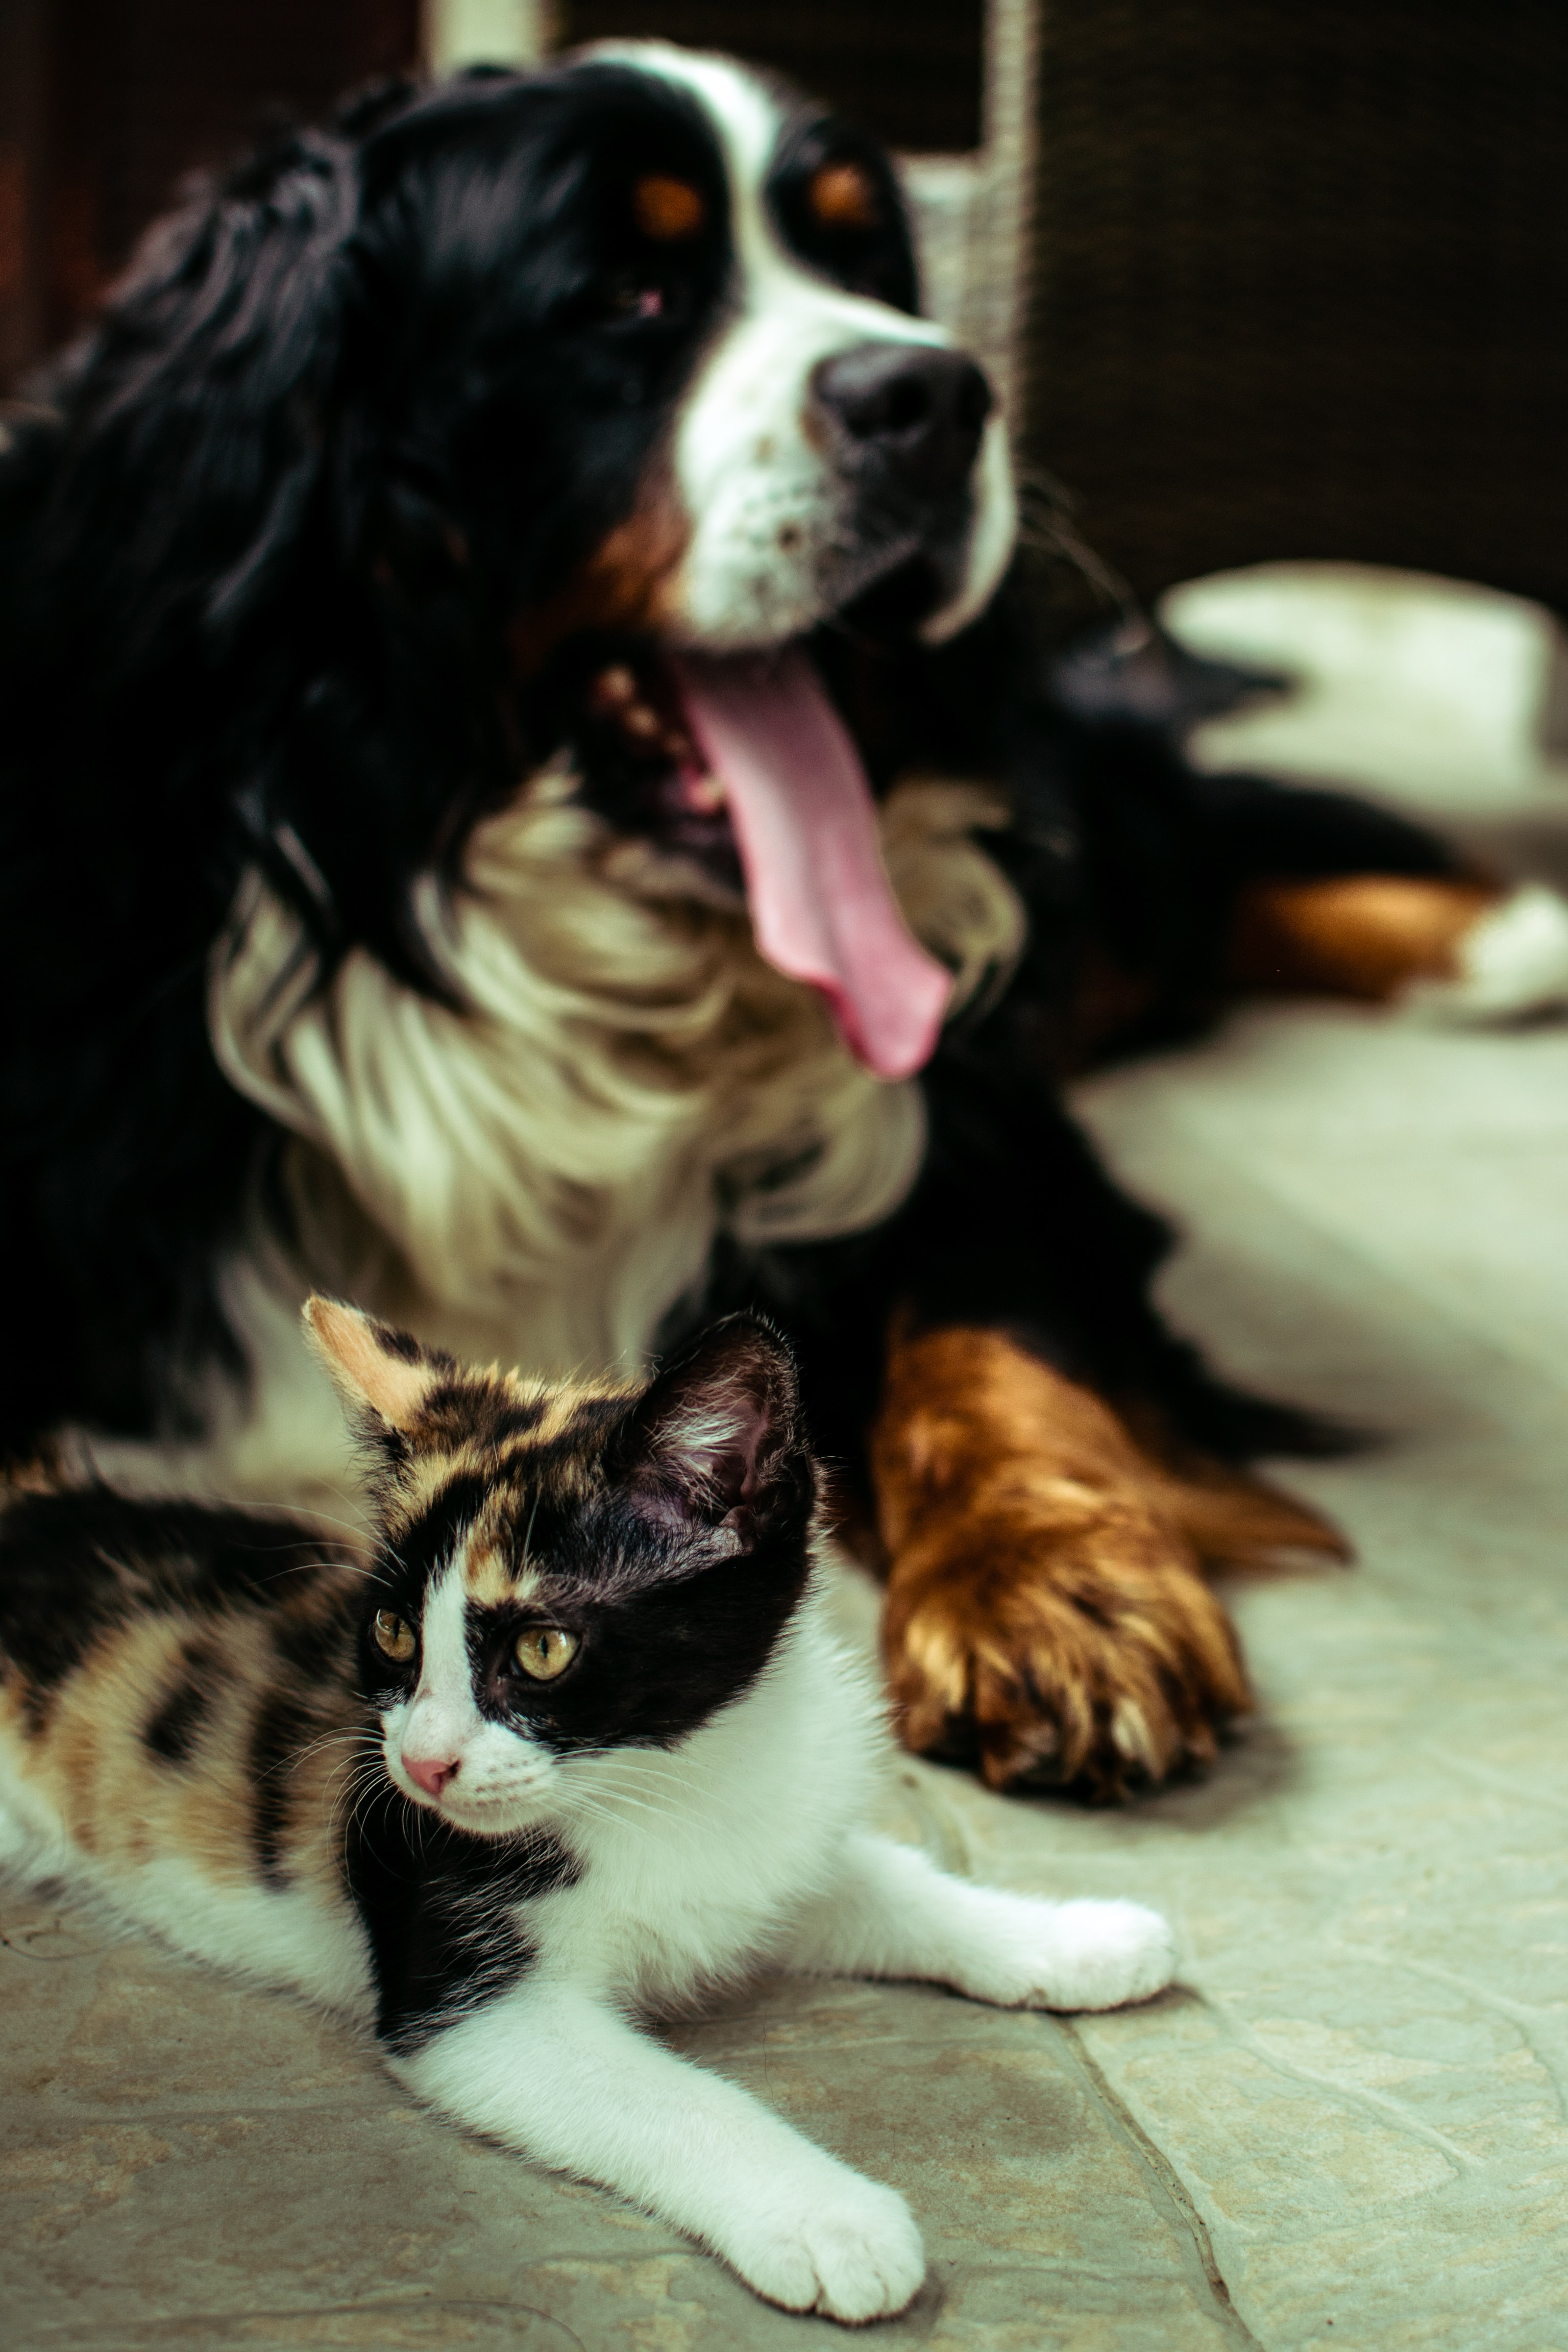
\includegraphics[width=0.8\linewidth]{img/jovana-askrabic-XYIQXLH_v0o-unsplash} \caption{Photo by Jovana Askrabic on Unsplash}\label{fig:photo}
\end{figure}

The goal of this assignment is to introduce you to R, RStudio, Git, and
GitHub, which you'll be using throughout the course both to learn the
data science concepts discussed in the course and to analyze real data
and come to informed conclusions.

\section{Getting started}\label{getting-started}

\subsection{Prerequisites}\label{prerequisites}

This assignment assumes that you have reviewed the lectures titled
``Meet the toolkit: Programming'' and ``Meet the toolkit: version
control and collaboration''. If you haven't yet done so, please pause
and complete the following before continuing.

\subsection{Terminology}\label{terminology}

We've already thrown around a few new terms, so let's define them before
we proceed.

\begin{itemize}
\tightlist
\item
  \textbf{R:} Name of the programming language we will be using
  throughout the course.
\item
  \textbf{RStudio:} An integrated development environment for R. In
  other words, a convenient interface for writing and running R code.
\item
  \textbf{Git:} A version control system.
\item
  \textbf{GitHub:} A web platform for hosting version controlled files
  and facilitating collaboration among users.
\item
  \textbf{Repository:} A Git repository contains all of your project's
  files and stores each file's revision history. It's common to refer to
  a repository as a repo.

  \begin{itemize}
  \tightlist
  \item
    In this course, each assignment you work on will be contained in a
    Git repo.
  \item
    For individual assignments, only you will have access to the repo.
    For team assignments, all team members will have access to a single
    repo where they work collaboratively.
  \item
    All repos associated with this course are housed in the course
    GitHub organization. The organization is set up such that students
    can only see repos they have access to, but the course staff can see
    all of them.
  \end{itemize}
\end{itemize}

\subsection{Starting slow}\label{starting-slow}

As the course progresses, you are encouraged to explore beyond what the
assignments dictate; a willingness to experiment will make you a much
better programmer! Before we get to that stage, however, you need to
build some basic fluency in R. First, we will explore the fundamental
building blocks of all of these tools.

Before you can get started with the analysis, you need to make sure you:

\begin{itemize}
\tightlist
\item
  have a GitHub account
\item
  are a member of the course GitHub organization
\item
  are a member of the course RStudio Cloud space
\end{itemize}

If you failed to confirm any of these, it means you have not yet
completed the prerequisites for this assignment. Please go back to
\hyperref[prerequisites]{Prerequisites} and complete them before
continuing the assignment.

\section{Workflow}\label{workflow}

\begin{Shaded}
\begin{Highlighting}[]
\NormalTok{**IMPORTANT:** If there is no GitHub repo created for you for this assignment, it means I didn\textquotesingle{}t have your GitHub username as of when I assigned the homework. Please let me know your GitHub username asap, and I can create your repo.}
\end{Highlighting}
\end{Shaded}

For each assignment in this course you will start with a GitHub repo
that I created for you and that contains the starter documents you will
build upon when working on your assignment. The first step is always to
bring these files into RStudio so that you can edit them, run them, view
your results, and interpret them. This action is called
\textbf{cloning}.

Then you will work in RStudio on the data analysis, making
\textbf{commits} along the way (snapshots of your changes) and finally
\textbf{push} all your work back to GitHub.

The next few steps will walk you through the process of getting
information of the repo to be cloned, cloning your repo in a new RStudio
Cloud project, and getting started with the analysis.

\subsubsection{Step 1. Get URL of repo to be
cloned}\label{step-1.-get-url-of-repo-to-be-cloned}

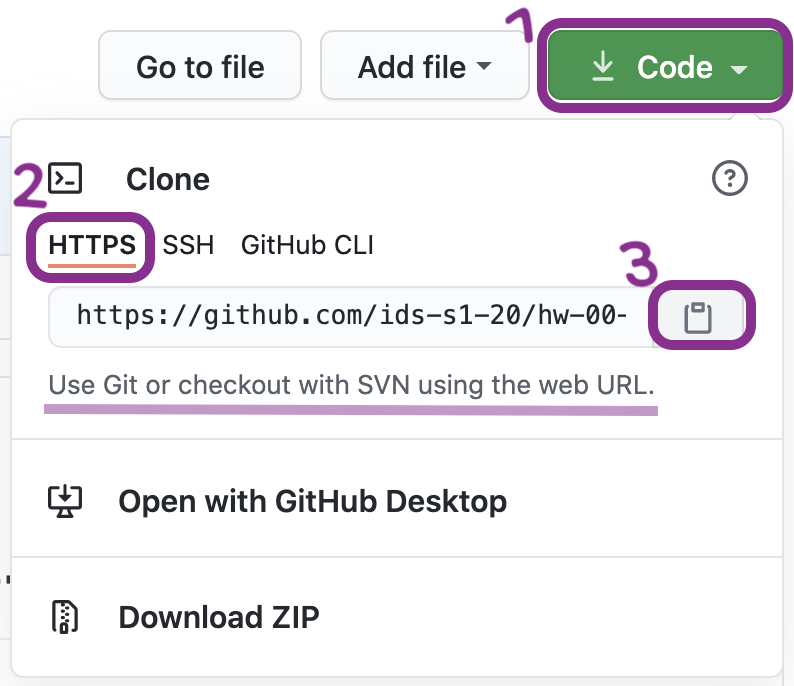
\includegraphics[width=0.8\linewidth]{img/clone-repo-link}

On GitHub, click on the green \textbf{Code} button, select
\textbf{HTTPS} (this might already be selected by default, and if it is,
you'll see the text \emph{Use Git or checkout with SVN using the web
URL} jas in the image on the right). Click on the clipboard icon 📋 to
copy the repo URL.

\subsubsection{Step 2. Go to RStudio
Cloud}\label{step-2.-go-to-rstudio-cloud}

Go to \href{https://posit.cloud/}{posit.cloud} and then \textbf{navigate
to the course workspace} via the left sidebar. It's very important that
you do this for two reasons:

\begin{itemize}
\tightlist
\item
  It's only when you're in the course workspace that you'll be able to
  benefit from R packages I've pre-installed for you so that your
  project can be configured correctly.
\item
  It's only when you're in the course workspace that your usage of
  RStudio Cloud won't count towards the free usage limits.
\end{itemize}


\includegraphics[width=0.8\linewidth]{img/course-workspace}

Before you proceed, confirm that you are in the course workspace by
checking out what's on your top bar in RStudio Cloud.

\subsubsection{Step 3. Clone the repo}\label{step-3.-clone-the-repo}

In RStudio, click on the \textbf{down arrow} next to New Project and
then choose \textbf{New Project from Git Repository}.

In the pop-up window, \textbf{paste the URL} you copied from GitHub,
make sure the box for \textbf{Add packages from the base project} is
checked (it should be, by default) and then click \textbf{OK}.

\begin{flushleft}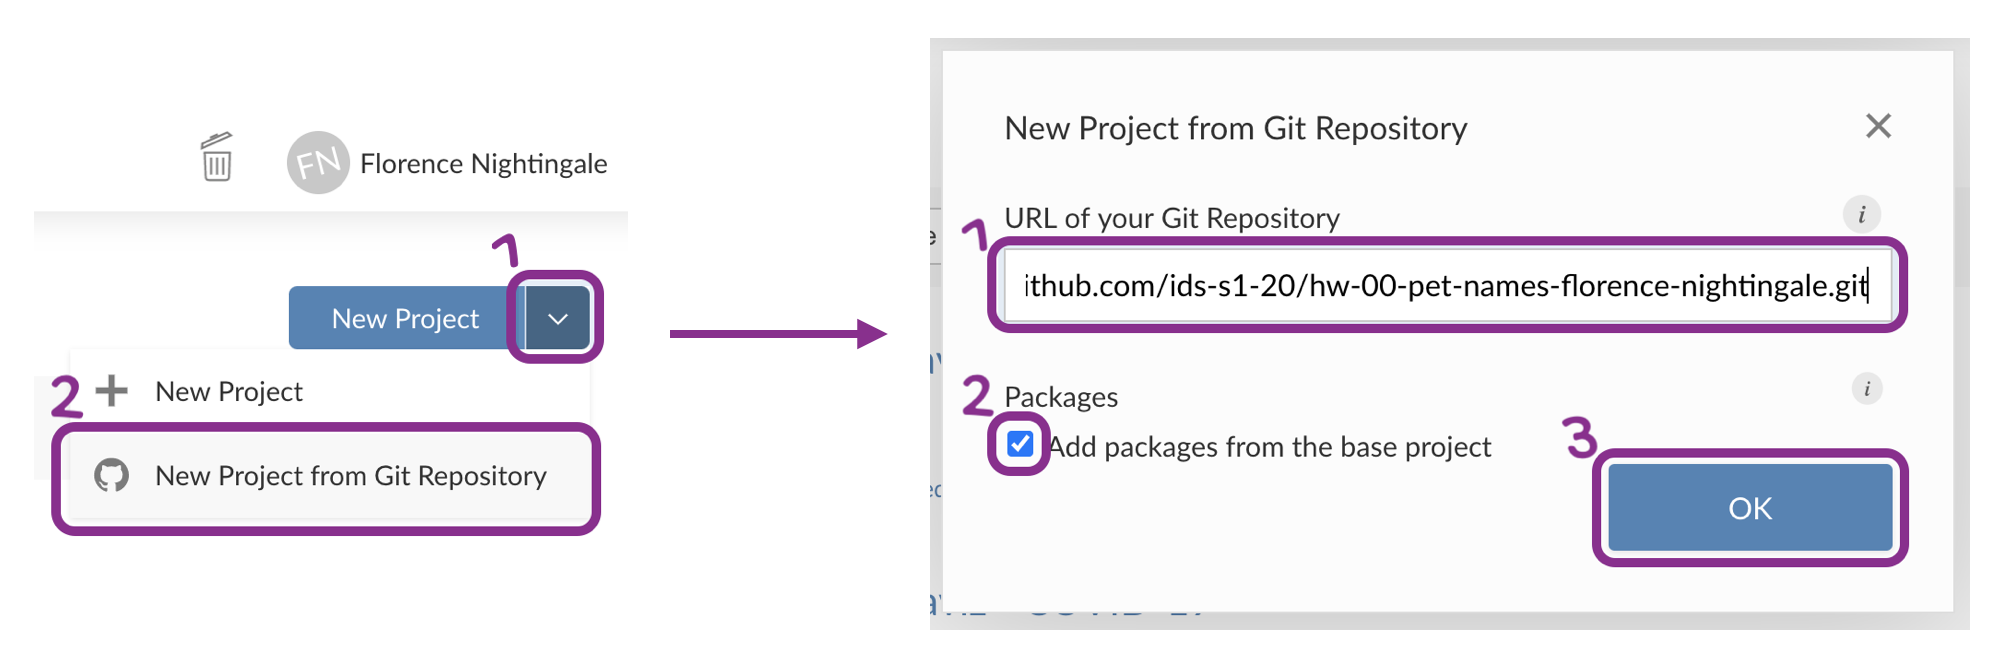
\includegraphics[width=0.8\linewidth]{img/new-project-from-git} \end{flushleft}

\section{Hello RStudio!}\label{hello-rstudio}

RStudio is comprised of four panes.

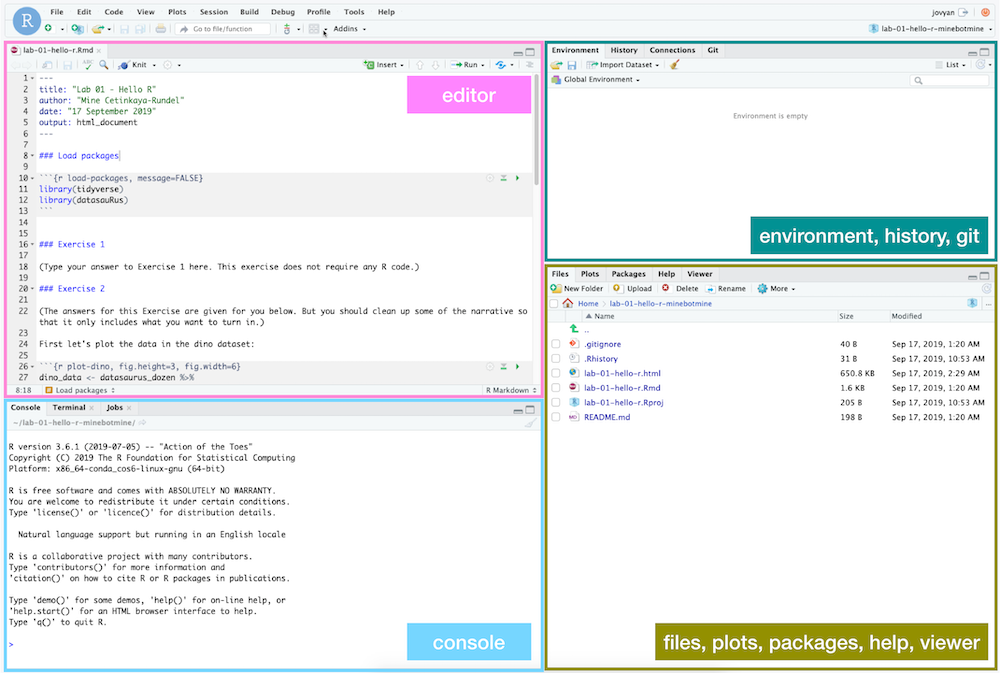
\includegraphics[width=0.8\linewidth]{img/rstudio-anatomy}

\begin{itemize}
\tightlist
\item
  On the bottom left is the Console, this is where you can write code
  that will be evaluated. Try typing \texttt{2\ +\ 2} here and hit
  enter, what do you get?
\item
  On the bottom right is the Files pane, as well as other panes that
  will come handy as we start our analysis.
\item
  If you click on a file, it will open in the editor, on the top left
  pane.
\item
  Finally, the top right pane shows your Environment. If you define a
  variable it would show up there. Try typing
  \texttt{x\ \textless{}-\ 2} in the Console and hit enter, what do you
  get in the \textbf{Environment} pane? Importantly, this pane is also
  where the \textbf{Git} interface lives. We will be using that
  regularly throughout this assignment.
\end{itemize}

\section{Warm up}\label{warm-up}

Before we introduce the data, let's warm up with some simple exercises.

\begin{Shaded}
\begin{Highlighting}[]
\NormalTok{The top portion of your R Markdown file (between the three dashed lines) is called **YAML**. It stands for "YAML Ain\textquotesingle{}t Markup Language". It is a human friendly data serialization standard for all programming languages. All you need to know is that this area is called the YAML (we will refer to it as such) and that it contains meta information about your document.}
\end{Highlighting}
\end{Shaded}

\subsection{Step 1. Update the YAML}\label{step-1.-update-the-yaml}

Open the R Markdown (Rmd) file in your project, change the author name
to your name, and knit the document.

\begin{center}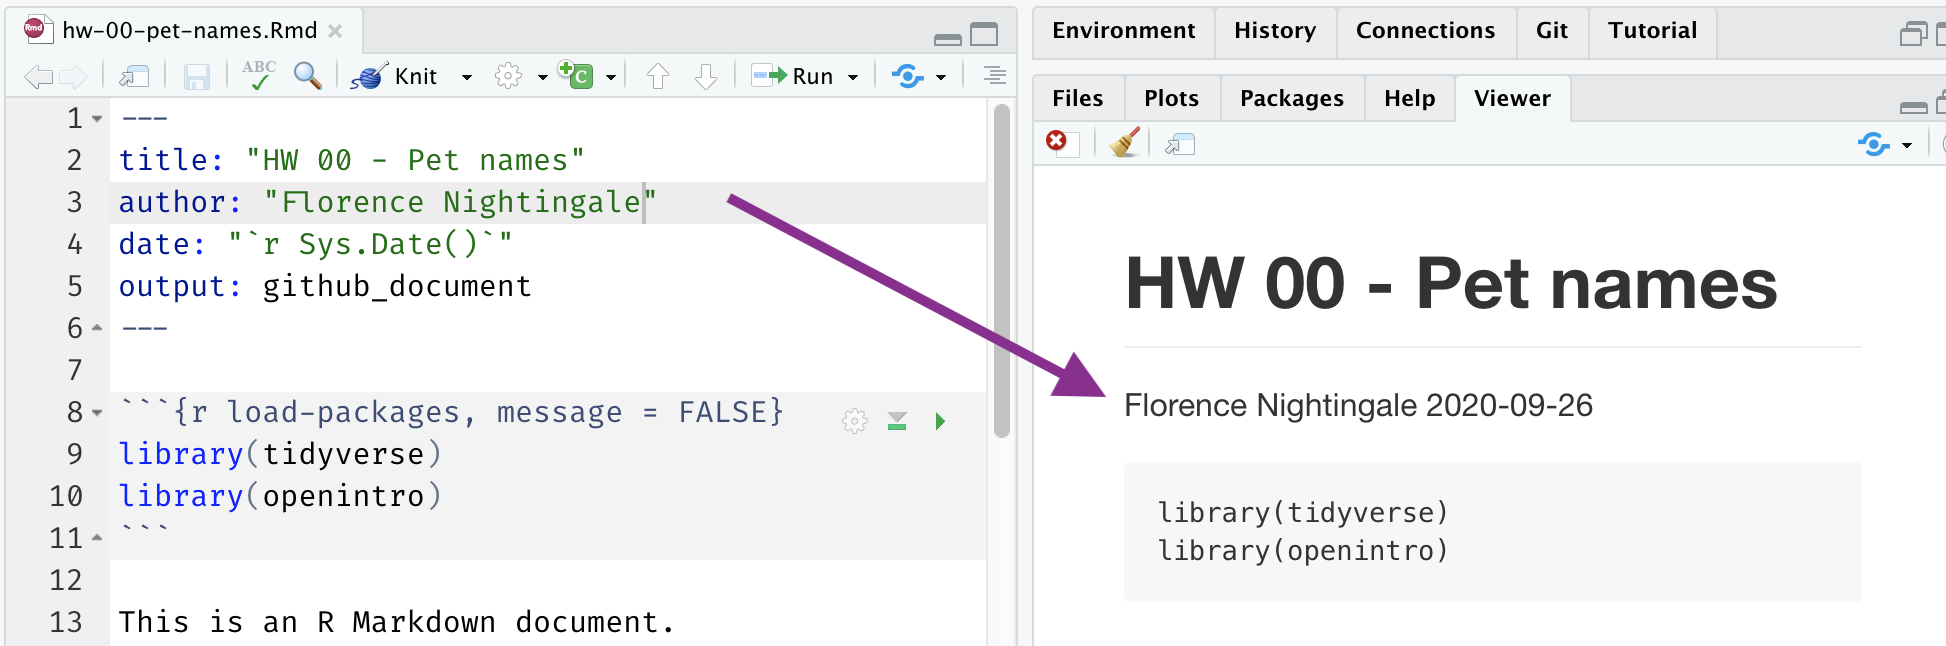
\includegraphics[width=0.8\linewidth]{img/yaml-raw-to-rendered} \end{center}

\subsection{Step 2: Commit}\label{step-2-commit}

Then Go to the \textbf{Git pane} in your RStudio.

You should see that your Rmd (R Markdown) file and its output, your md
file (Markdown), are listed there as recently changed files.

Next, click on \textbf{Diff}. This will pop open a new window that shows
you the \textbf{diff}erence between the last committed state of the
document and its current state that includes your changes. If you're
happy with these changes, click on the checkboxes of all files in the
list, and type \emph{``Update author name''} in the \textbf{Commit
message} box and hit \textbf{Commit}.

\begin{flushleft}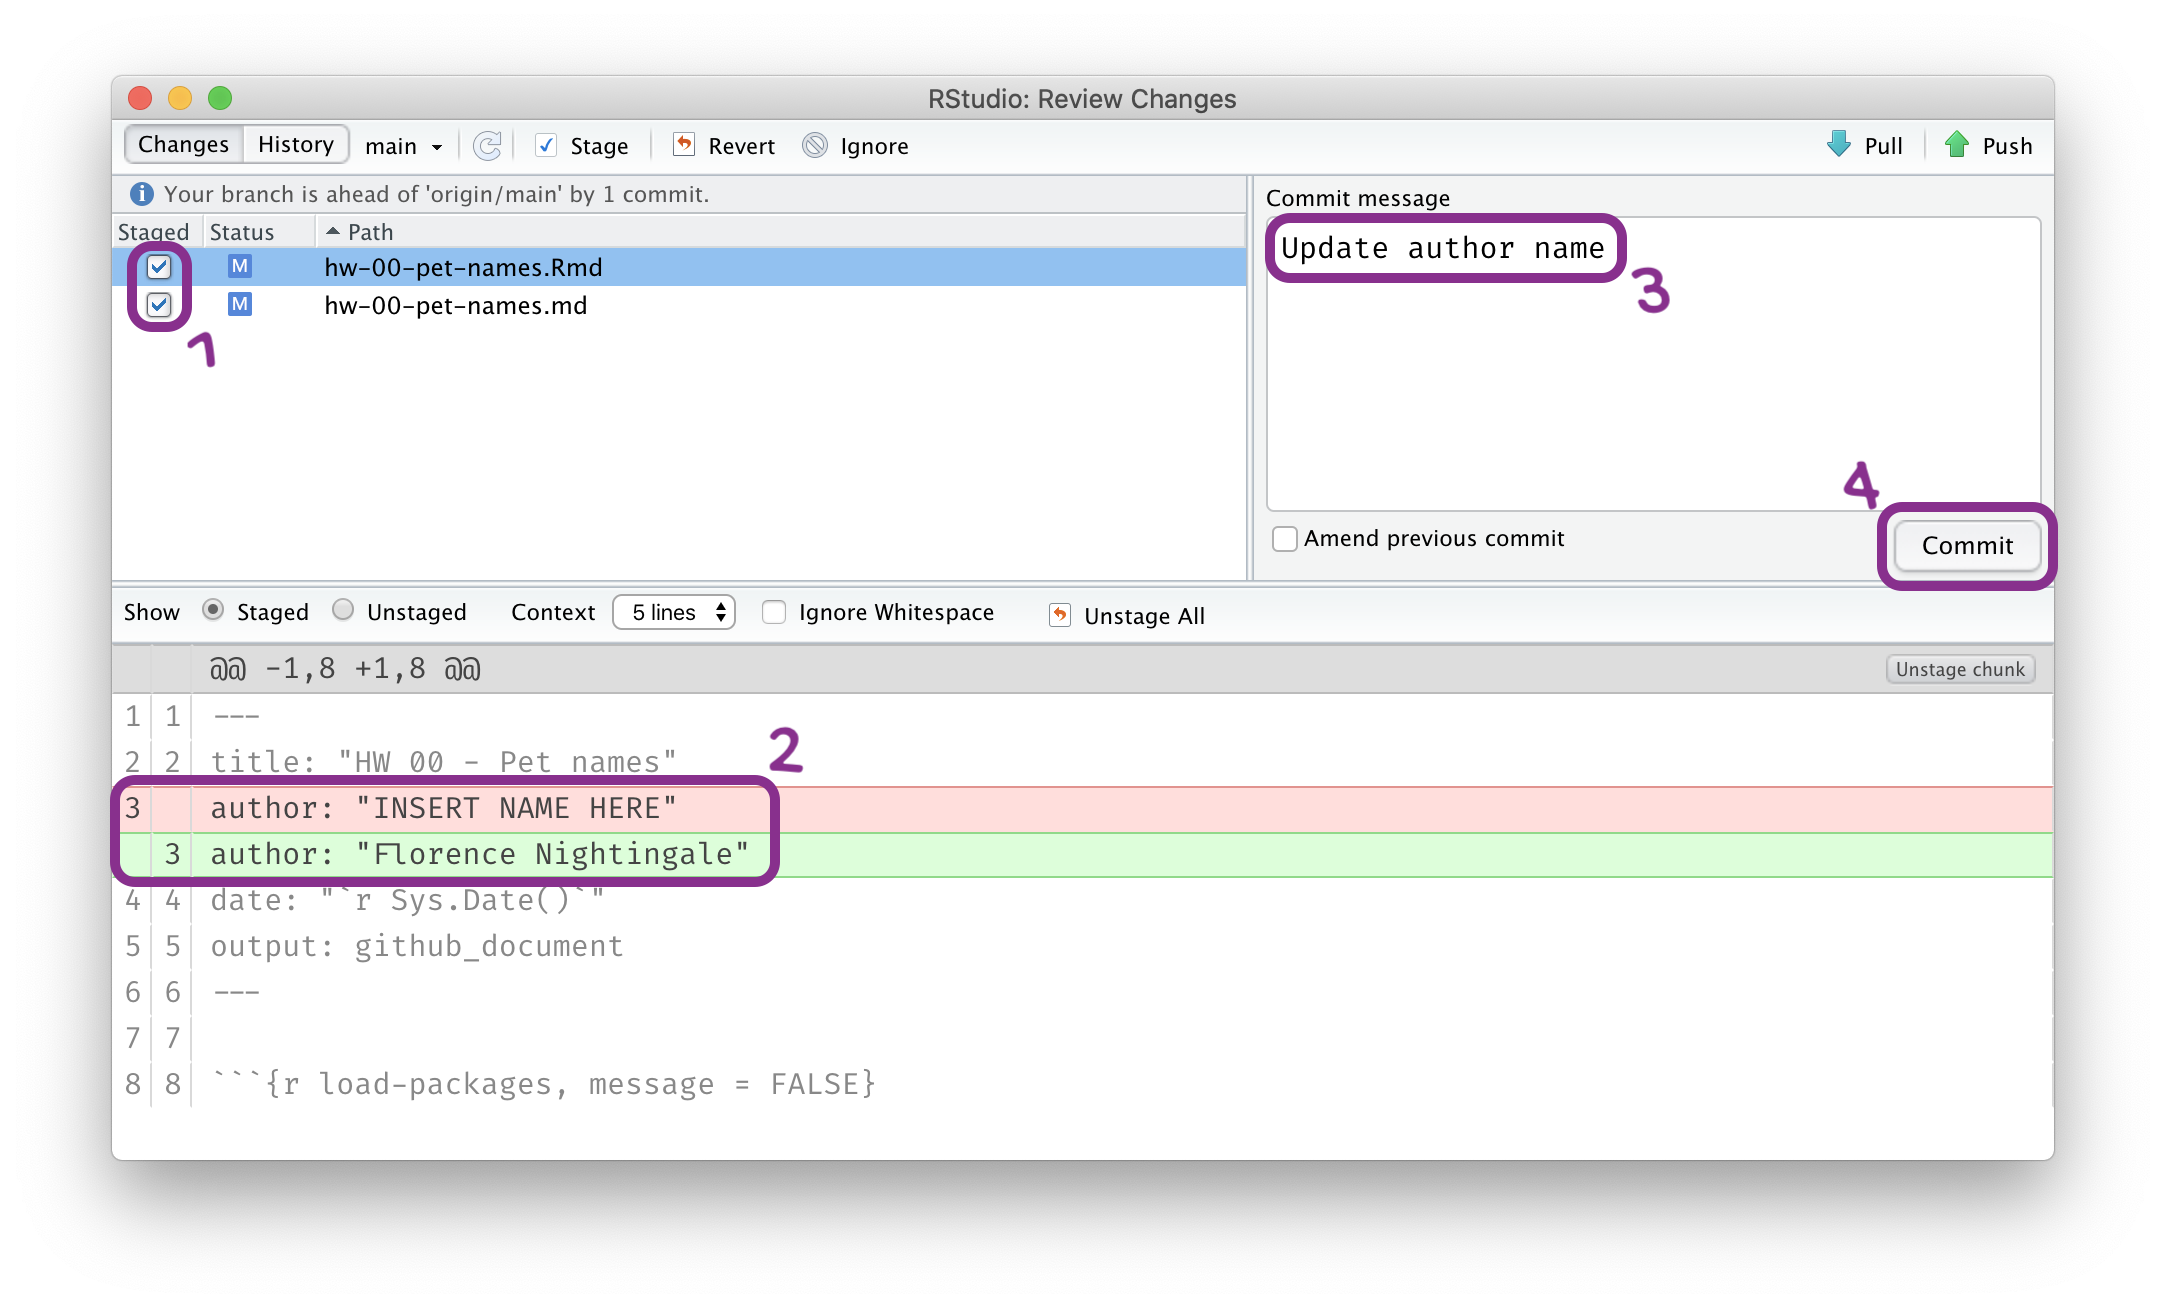
\includegraphics[width=0.8\linewidth]{img/update-author-name-commit} \end{flushleft}

You don't have to commit after every change, this would get quite
cumbersome. You should consider committing states that are
\emph{meaningful to you} for inspection, comparison, or restoration. In
the first few assignments we will tell you exactly when to commit and in
some cases, what commit message to use. As the semester progresses we
will let you make these decisions.

\subsection{Step 3. Push}\label{step-3.-push}

Now that you have made an update and committed this change, it's time to
push these changes to the web! Or more specifically, to your repo on
GitHub. Why? So that others can see your changes. And by others, we mean
the course teaching team (your repos in this course are private to you
and us, only). In order to push your changes to GitHub, click on
\textbf{Push}.

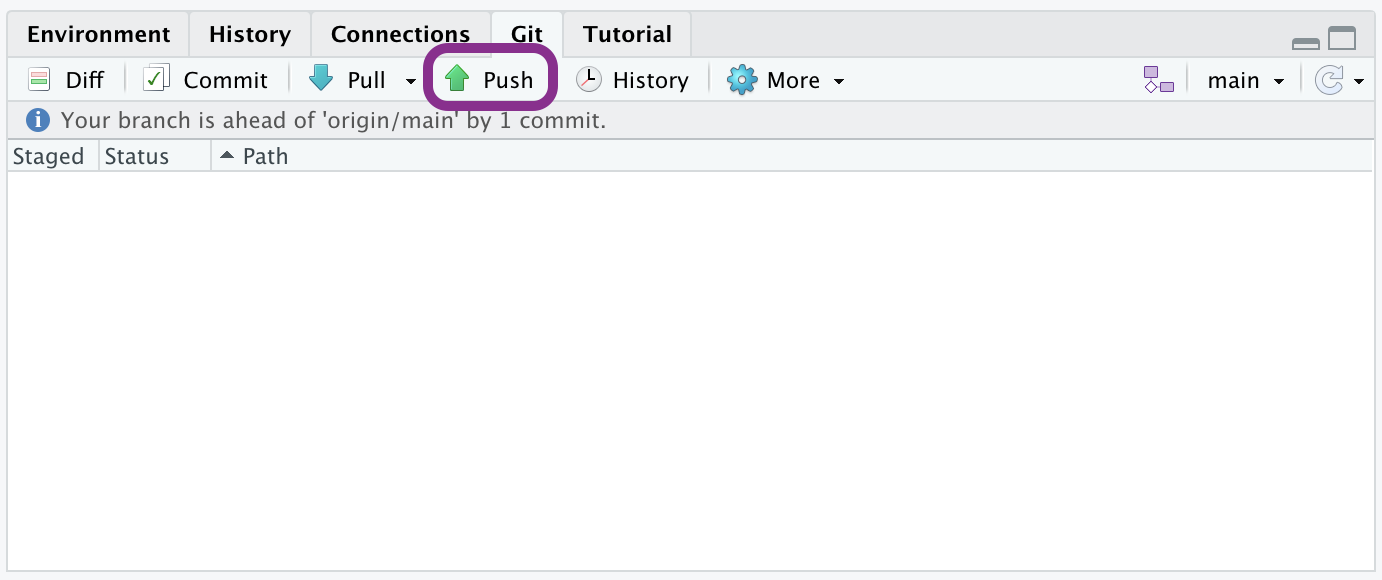
\includegraphics[width=0.8\linewidth]{img/ready-to-push}

This will prompt a dialogue box where you first need to enter your user
name, and then your password. This might feel cumbersome. Bear with
me\ldots{} I \emph{will} teach you how to save your password so you
don't have to enter it every time. But for this one assignment you'll
have to manually enter each time you push in order to gain some
experience with it.

\textbf{Thought exercise:} Which of the above steps (updating the YAML,
committing, and pushing) needs to talk to GitHub?\footnote{Only pushing
  requires talking to GitHub, this is why you're asked for your password
  at that point.}

Updating the YAML is also a local operation, it doesn't require any
communication with GitHub. Committing is a local operation, it doesn't
require any communication with GitHub. Pushing requires communication
with GitHub, as it is the step that sends your changes to GitHub.

\section{Packages}\label{packages}

R is an open-source language, and developers contribute functionality to
R via packages. In this assignment we will use the following packages:

\begin{itemize}
\tightlist
\item
  \textbf{tidyverse}: a collection of packages for doing data analysis
  in a ``tidy'' way
\item
  \textbf{openintro}: a package that contains the datasets from
  OpenIntro resources
\end{itemize}

We use the \texttt{library()} function to load packages. In your R
Markdown document you should see an R chunk labelled
\texttt{load-packages} which has the necessary code for loading both
packages. You should also load these packages in your Console, which you
can do by sending the code to your Console by clicking on the
\textbf{Run Current Chunk} icon (green arrow pointing right icon).

\begin{flushleft}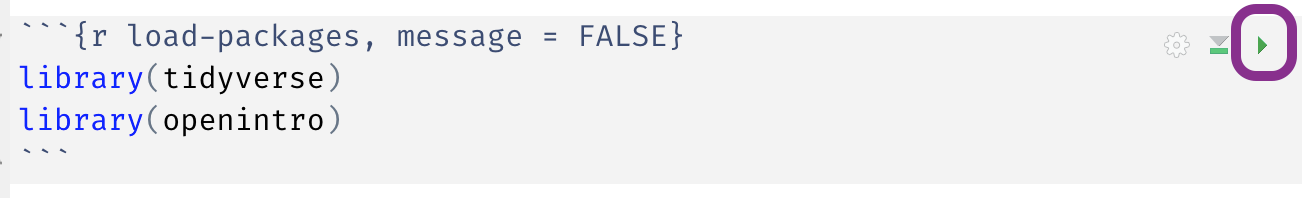
\includegraphics[width=0.8\linewidth]{img/load-packages-chunk} \end{flushleft}

Note that these packages also get loaded in your R Markdown environment
when you \textbf{Knit} your R Markdown document.

\section{Data}\label{data}

The city of \href{https://en.wikipedia.org/wiki/Seattle}{Seattle, WA}
has an open data portal that includes pets registered in the city. For
each registered pet, we have information on the pet's name and species.
The data used in this exercise can be found in the \textbf{openintro}
package, and it's called \texttt{seattlepets}. Since the dataset is
distributed with the package, we don't need to load it separately; it
becomes available to us when we load the package.

You can view the dataset as a spreadsheet using the \texttt{View()}
function. Note that you should not put this function in your R Markdown
document, but instead type it directly in the Console, as it pops open a
new window (and the concept of popping open a window in a static
document doesn't really make sense\ldots). When you run this in the
console, you'll see the following \textbf{data viewer} window pop up.

\begin{Shaded}
\begin{Highlighting}[]
\FunctionTok{View}\NormalTok{(seattlepets)}
\end{Highlighting}
\end{Shaded}

\begin{flushleft}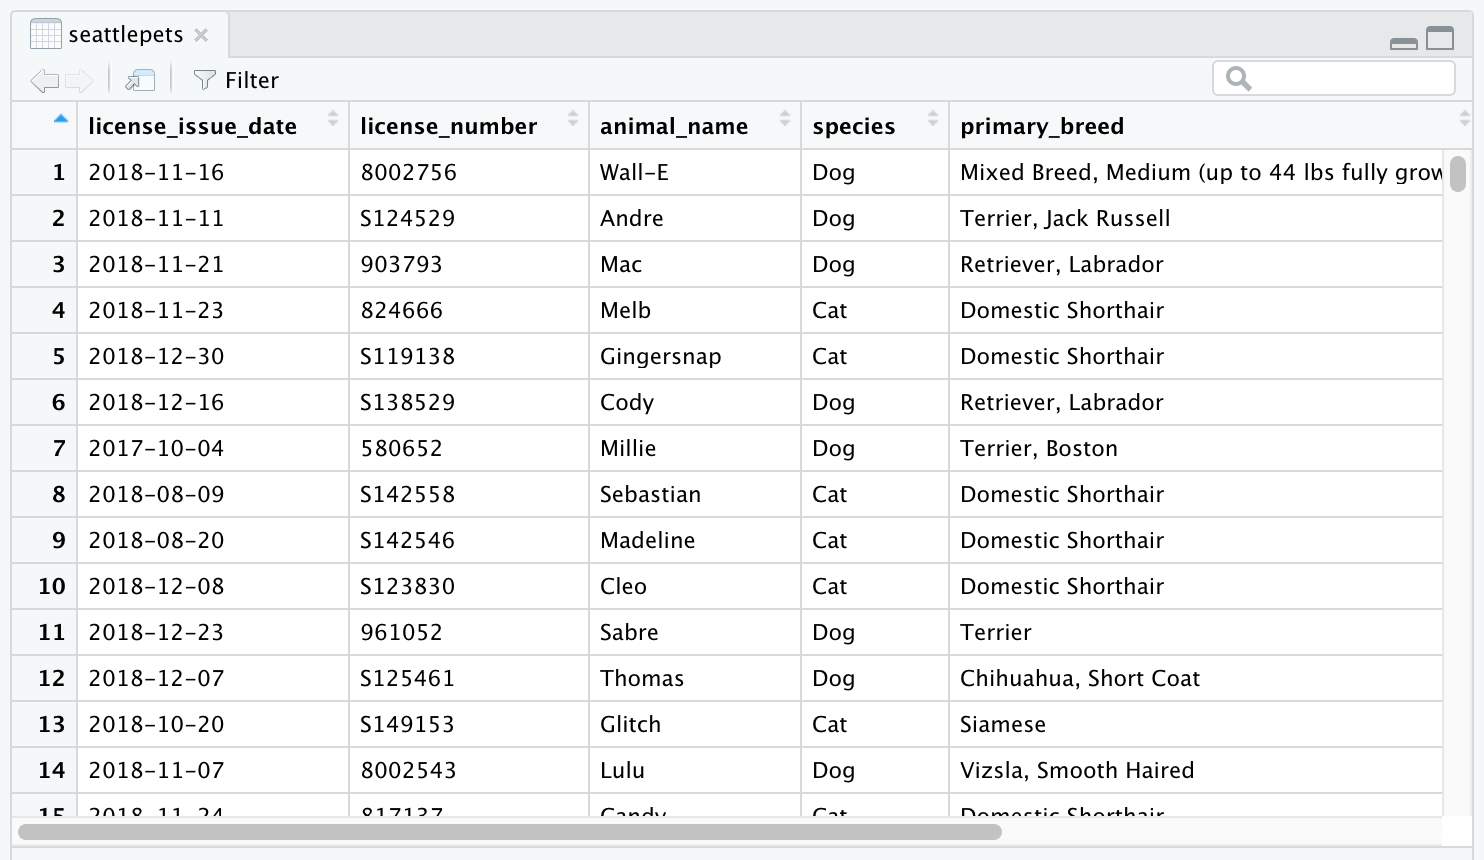
\includegraphics[width=0.8\linewidth]{img/view-data} \end{flushleft}

You can find out more about the dataset by inspecting its documentation
(which contains a \textbf{data dictionary}, name of each variable and
its description), which you can access by running \texttt{?seattlepets}
in the Console or using the Help menu in RStudio to search for
\texttt{seattlepets}.

By running \texttt{?seattlepets} in the Console or using the Help menu
in RStudio to search for \texttt{seattlepets}, you'll see documentation
about the dataset pop up in the Help pane which contains information
such as the source of the data, a brief description, and a data
dictionary that describes each variable in the dataset.

\section{Exercises}\label{exercises}

\subsection{Exercise \#1}\label{exercise-1}

According to the data dictionary, how many pets are included in this
dataset?

There are a total of 52,519 pets in the dataset with 7 variables for
each pet.

\begin{Shaded}
\begin{Highlighting}[]
\CommentTok{\# Get the number of entries (rows) and variables (columns)}
\FunctionTok{nrow}\NormalTok{(seattlepets)}
\end{Highlighting}
\end{Shaded}

\begin{verbatim}
## [1] 52519
\end{verbatim}

\begin{Shaded}
\begin{Highlighting}[]
\FunctionTok{ncol}\NormalTok{(seattlepets)}
\end{Highlighting}
\end{Shaded}

\begin{verbatim}
## [1] 7
\end{verbatim}

🧶 ✅ ⬆️ \emph{Write your answer in your R Markdown document under
Exercise 1, knit the document, commit your changes with a commit message
that says ``Completed Exercise 1'', and push. Make sure to commit and
push all changed files so that your Git pane is cleared up afterwards.}

\subsection{Exercise \#2}\label{exercise-2}

Again, according to the data dictionary, how many variables do we have
for each pet?

There are 7 variables for each pet in the dataset:

\begin{itemize}
\item
  \texttt{license\_issue\_date}: Date the animal was registered with
  Seattle
\item
  \texttt{license\_number}: Unique identifier for each pet license
\item
  \texttt{animal\_name}: Name of the pet
\item
  \texttt{species}: Species of the pet (e.g., Dog, Cat, etc.)
\item
  \texttt{primary\_breed}: Primary breed of the pet
\item
  \texttt{secondary\_breed}: Secondary breed of the pet (if applicable)
\item
  \texttt{zip\_code}: Zip code animal is registered in
\end{itemize}

\begin{Shaded}
\begin{Highlighting}[]
\FunctionTok{colnames}\NormalTok{(seattlepets)}
\end{Highlighting}
\end{Shaded}

\begin{verbatim}
## [1] "license_issue_date" "license_number"     "animal_name"       
## [4] "species"            "primary_breed"      "secondary_breed"   
## [7] "zip_code"
\end{verbatim}

🧶 ✅ ⬆️ \emph{Write your answer in your R Markdown document under
Exercise 2, knit the document, commit your changes with a commit message
that says ``Completed Exercise 2'', and push. Make sure to commit and
push all changed files so that your Git pane is cleared up afterwards.}

\subsection{Exercise \#3}\label{exercise-3}

What are the three most common pet names in Seattle?

The most common pet names are \emph{Lucy}, \emph{Charlie}, and
\emph{Luna}.

To do this you will need to count the frequencies of each pet name and
display the results in descending order of frequency so that you can
easily see the top three most popular names. The following code does
exactly that.

\begin{Shaded}
\begin{Highlighting}[]
\NormalTok{The two lines of code can be read as "Start with the seattlepets data frame, and then count the animal\_names, and display the results sorted in descending order. The \textquotesingle{}and then\textquotesingle{} in the previous sentence maps to \%\textgreater{}\%, the pipe operator, which takes what comes before it and plugs it in as the first argument of the function that comes after it."}
\end{Highlighting}
\end{Shaded}

The code below takes the \texttt{seattlepets} dataset from the
\textbf{openintro} package and produces a frequency table of pet names.
It first standardizes the \texttt{animal\_name} variable by converting
all names to lowercase and trimming any leading or trailing spaces. It
then removes missing (\texttt{NA}) or blank entries to ensure only valid
names remain. Finally, it counts the occurrences of each unique name,
sorts them from most to least common, and labels the frequency column as
\texttt{count} for clarity.

\begin{Shaded}
\begin{Highlighting}[]
\NormalTok{popular\_names }\OtherTok{\textless{}{-}}\NormalTok{ seattlepets }\SpecialCharTok{\%\textgreater{}\%}
  \FunctionTok{mutate}\NormalTok{(}\AttributeTok{animal\_name =}\NormalTok{ animal\_name }\SpecialCharTok{|\textgreater{}}
    \FunctionTok{tolower}\NormalTok{() }\SpecialCharTok{|\textgreater{}}
    \FunctionTok{trimws}\NormalTok{()) }\SpecialCharTok{\%\textgreater{}\%} \CommentTok{\# remove leading/trailing spaces}
  \FunctionTok{filter}\NormalTok{(}\SpecialCharTok{!}\FunctionTok{is.na}\NormalTok{(animal\_name), animal\_name }\SpecialCharTok{!=} \StringTok{""}\NormalTok{) }\SpecialCharTok{\%\textgreater{}\%}
  \FunctionTok{count}\NormalTok{(animal\_name, }\AttributeTok{sort =} \ConstantTok{TRUE}\NormalTok{, }\AttributeTok{name =} \StringTok{"count"}\NormalTok{)}
\NormalTok{popular\_names}
\end{Highlighting}
\end{Shaded}

\begin{verbatim}
## # A tibble: 13,775 x 2
##    animal_name count
##    <chr>       <int>
##  1 lucy          440
##  2 charlie       387
##  3 luna          357
##  4 bella         331
##  5 max           273
##  6 daisy         261
##  7 molly         240
##  8 jack          232
##  9 lily          232
## 10 stella        227
## # i 13,765 more rows
\end{verbatim}

\begin{Shaded}
\begin{Highlighting}[]
\FunctionTok{head}\NormalTok{(popular\_names, }\DecValTok{3}\NormalTok{)}
\end{Highlighting}
\end{Shaded}

\begin{verbatim}
## # A tibble: 3 x 2
##   animal_name count
##   <chr>       <int>
## 1 lucy          440
## 2 charlie       387
## 3 luna          357
\end{verbatim}

🧶 ✅ ⬆️ \emph{Write your answer in your R Markdown document under
Exercise 3. In this exercise you will not only provide a written answer
but also include some code and output. You should insert the code in the
code chunk provided for you, knit the document to see the output, and
then write your narrative for the answer based on the output of this
function, and knit again to see your narrative, code, and output in the
resulting document. Then, commit your changes with a commit message that
says ``Completed Exercise 3'', and push. Make sure to commit and push
all changed files so that your Git pane is cleared up afterwards.}

Let's also look to see what the most common pet names are for various
species. For this we need to first \texttt{group\_by()} the
\texttt{species}, and then do the same counting we did before.

\begin{Shaded}
\begin{Highlighting}[]
\NormalTok{Looks like many of those NAs were cats. Poor unnamed kitties…}
\end{Highlighting}
\end{Shaded}

\begin{Shaded}
\begin{Highlighting}[]
\NormalTok{seattlepets }\SpecialCharTok{\%\textgreater{}\%}
  \FunctionTok{group\_by}\NormalTok{(species) }\SpecialCharTok{\%\textgreater{}\%}
  \FunctionTok{count}\NormalTok{(animal\_name, }\AttributeTok{sort =} \ConstantTok{TRUE}\NormalTok{)}
\end{Highlighting}
\end{Shaded}

\begin{verbatim}
## # A tibble: 16,823 x 3
## # Groups:   species [4]
##    species animal_name     n
##    <chr>   <chr>       <int>
##  1 Cat     <NA>          406
##  2 Dog     Lucy          337
##  3 Dog     Charlie       306
##  4 Dog     Bella         249
##  5 Dog     Luna          244
##  6 Dog     Daisy         221
##  7 Dog     Cooper        189
##  8 Dog     Lola          187
##  9 Dog     Max           186
## 10 Dog     Molly         186
## # i 16,813 more rows
\end{verbatim}

But this output isn't exactly what we wanted. We wanted to know the most
common cat and dog names, but there are barely any cats present in this
output! This is because there are more dogs than cats in the dataset
overall. We can confirm this by counting the various species in the
data.

\begin{Shaded}
\begin{Highlighting}[]
\NormalTok{6 pigs in the city? Ok… But we\textquotesingle{}ll continue with cats and dogs.}
\end{Highlighting}
\end{Shaded}

\begin{Shaded}
\begin{Highlighting}[]
\NormalTok{seattlepets }\SpecialCharTok{\%\textgreater{}\%}
  \FunctionTok{count}\NormalTok{(species, }\AttributeTok{sort =} \ConstantTok{TRUE}\NormalTok{)}
\end{Highlighting}
\end{Shaded}

\begin{verbatim}
## # A tibble: 4 x 2
##   species     n
##   <chr>   <int>
## 1 Dog     35181
## 2 Cat     17294
## 3 Goat       38
## 4 Pig         6
\end{verbatim}

Let's search for the top 5 cat and dog names. To do this, we can use the
\texttt{slice\_max()} function. The first argument in the function is
the variable we want to select the highest values of, which is
\texttt{n}. The second argument is the number of rows to select, which
is \texttt{n\ =\ 5} for the top 5. It may be a bit confusing that both
of these are \texttt{n}, but this is because we already have a variable
called \texttt{n} in the data frame.

\begin{Shaded}
\begin{Highlighting}[]
\NormalTok{seattlepets }\SpecialCharTok{\%\textgreater{}\%}
  \FunctionTok{group\_by}\NormalTok{(species) }\SpecialCharTok{\%\textgreater{}\%}
  \FunctionTok{count}\NormalTok{(animal\_name, }\AttributeTok{sort =} \ConstantTok{TRUE}\NormalTok{) }\SpecialCharTok{\%\textgreater{}\%}
  \FunctionTok{slice\_max}\NormalTok{(n, }\AttributeTok{n =} \DecValTok{5}\NormalTok{)}
\end{Highlighting}
\end{Shaded}

\begin{verbatim}
## # A tibble: 53 x 3
## # Groups:   species [4]
##    species animal_name     n
##    <chr>   <chr>       <int>
##  1 Cat     <NA>          406
##  2 Cat     Luna          111
##  3 Cat     Lucy          102
##  4 Cat     Lily           86
##  5 Cat     Max            83
##  6 Dog     Lucy          337
##  7 Dog     Charlie       306
##  8 Dog     Bella         249
##  9 Dog     Luna          244
## 10 Dog     Daisy         221
## # i 43 more rows
\end{verbatim}

This output provides the top 5 names for each species along with their
respective counts. However, the results are sorted by count across all
species, which means that the top names for one species may appear
before those of another species.

\subsection{Exercise \#4}\label{exercise-4}

Based on the previous output we can easily identify the most common cat
and dog names in Seattle, but the output is sorted by \texttt{n} (the
frequencies) as opposed to being organized by the \texttt{species}.
Build on the pipeline to arrange the results so that they're arranged by
\texttt{species} first, and then \texttt{n}. This means you will need to
add one more step to the pipeline, and you have two options:
\texttt{arrange(species,\ n)} or \texttt{arrange(n,\ species)}. You
should try both and decide which one organizes the output by species and
then ranks the names in order of frequency for each species.

\begin{Shaded}
\begin{Highlighting}[]
\NormalTok{popular\_names }\OtherTok{\textless{}{-}}\NormalTok{ seattlepets }\SpecialCharTok{\%\textgreater{}\%}
  \FunctionTok{mutate}\NormalTok{(}\AttributeTok{animal\_name =}\NormalTok{ animal\_name }\SpecialCharTok{|\textgreater{}}
    \FunctionTok{tolower}\NormalTok{() }\SpecialCharTok{|\textgreater{}}
    \FunctionTok{trimws}\NormalTok{()) }\SpecialCharTok{\%\textgreater{}\%}
  \FunctionTok{filter}\NormalTok{(}\SpecialCharTok{!}\FunctionTok{is.na}\NormalTok{(animal\_name), animal\_name }\SpecialCharTok{!=} \StringTok{""}\NormalTok{) }\SpecialCharTok{\%\textgreater{}\%}
  \FunctionTok{count}\NormalTok{(species, animal\_name, }\AttributeTok{sort =} \ConstantTok{TRUE}\NormalTok{, }\AttributeTok{name =} \StringTok{"count"}\NormalTok{)}

\NormalTok{popular\_names}
\end{Highlighting}
\end{Shaded}

\begin{verbatim}
## # A tibble: 16,669 x 3
##    species animal_name count
##    <chr>   <chr>       <int>
##  1 Dog     lucy          338
##  2 Dog     charlie       306
##  3 Dog     bella         249
##  4 Dog     luna          246
##  5 Dog     daisy         221
##  6 Dog     cooper        189
##  7 Dog     max           189
##  8 Dog     lola          188
##  9 Dog     molly         186
## 10 Dog     stella        185
## # i 16,659 more rows
\end{verbatim}

\begin{Shaded}
\begin{Highlighting}[]
\NormalTok{popular\_names }\OtherTok{\textless{}{-}}\NormalTok{ popular\_names }\SpecialCharTok{\%\textgreater{}\%}
  \FunctionTok{group\_by}\NormalTok{(species) }\SpecialCharTok{\%\textgreater{}\%}
  \FunctionTok{arrange}\NormalTok{(species, }\FunctionTok{desc}\NormalTok{(count), animal\_name)}
\NormalTok{popular\_names}
\end{Highlighting}
\end{Shaded}

\begin{verbatim}
## # A tibble: 16,669 x 3
## # Groups:   species [4]
##    species animal_name count
##    <chr>   <chr>       <int>
##  1 Cat     luna          111
##  2 Cat     lucy          102
##  3 Cat     lily           86
##  4 Cat     max            83
##  5 Cat     bella          82
##  6 Cat     charlie        81
##  7 Cat     oliver         73
##  8 Cat     jack           65
##  9 Cat     sophie         59
## 10 Cat     leo            54
## # i 16,659 more rows
\end{verbatim}

\begin{Shaded}
\begin{Highlighting}[]
\CommentTok{\# Select the top 10 most common pet names for each species and display their counts}
\NormalTok{top\_species\_names }\OtherTok{\textless{}{-}}\NormalTok{ popular\_names }\SpecialCharTok{\%\textgreater{}\%}
  \FunctionTok{group\_by}\NormalTok{(species) }\SpecialCharTok{\%\textgreater{}\%}
  \FunctionTok{slice\_max}\NormalTok{(}\AttributeTok{order\_by =}\NormalTok{ count, }\AttributeTok{n =} \DecValTok{10}\NormalTok{, }\AttributeTok{with\_ties =} \ConstantTok{FALSE}\NormalTok{)}
\NormalTok{top\_species\_names}
\end{Highlighting}
\end{Shaded}

\begin{verbatim}
## # A tibble: 35 x 3
## # Groups:   species [4]
##    species animal_name count
##    <chr>   <chr>       <int>
##  1 Cat     luna          111
##  2 Cat     lucy          102
##  3 Cat     lily           86
##  4 Cat     max            83
##  5 Cat     bella          82
##  6 Cat     charlie        81
##  7 Cat     oliver         73
##  8 Cat     jack           65
##  9 Cat     sophie         59
## 10 Cat     leo            54
## # i 25 more rows
\end{verbatim}

Here, we can see the top 10 names for each species along with their
counts, organized by species and then by frequency within each species.

Looking at the data more closely:

\begin{enumerate}
\def\labelenumi{\arabic{enumi}.}
\item
  \textbf{Dogs}: The most popular dog names are ``lucy'' (338),
  ``charlie'' (306), and ``bella'' (249). These three names
  significantly outrank other dog names, with counts over 200. There's a
  gradual decline in popularity after the top three names.
\item
  \textbf{Cats}: The most popular cat names are ``luna'' (111), ``lucy''
  (102), and ``lily'' (86). Cat names show a more even distribution in
  popularity compared to dog names, with a more gradual decrease in
  frequency from top to bottom.
\item
  \textbf{Goats}: All goat names appear just once in the dataset,
  suggesting there are few registered goats in Seattle, and their names
  are quite diverse with no clear pattern of popularity.
\item
  \textbf{Pigs}: Similar to goats, all pig names appear only once,
  indicating a small population of registered pigs with unique names.
\end{enumerate}

It's interesting to note that ``lucy'' appears in the top names for both
cats and dogs, showing some cross-species name preferences. The data
also reveals that dogs are much more commonly registered pets in Seattle
than cats, as evidenced by the higher counts for dog names compared to
cat names.

Now that we have the top 10 names for each species, we can create a
contingency table that displays the counts of these names across
different species.

\begin{Shaded}
\begin{Highlighting}[]
\CommentTok{\# Start from popular\_names (species, animal\_name, count)}
\NormalTok{contingency\_tbl }\OtherTok{\textless{}{-}}\NormalTok{ top\_species\_names }\SpecialCharTok{\%\textgreater{}\%}
  \FunctionTok{pivot\_wider}\NormalTok{(}
    \AttributeTok{names\_from =}\NormalTok{ species, }\CommentTok{\# columns become species}
    \AttributeTok{values\_from =}\NormalTok{ count, }\CommentTok{\# values are counts}
    \AttributeTok{values\_fill =} \ConstantTok{NA} \CommentTok{\# fill missing combos with 0}
\NormalTok{  )}
\NormalTok{contingency\_tbl}
\end{Highlighting}
\end{Shaded}

\begin{verbatim}
## # A tibble: 30 x 5
##    animal_name   Cat   Dog  Goat   Pig
##    <chr>       <int> <int> <int> <int>
##  1 luna          111   246    NA    NA
##  2 lucy          102   338    NA    NA
##  3 lily           86    NA    NA    NA
##  4 max            83   189    NA    NA
##  5 bella          82   249    NA    NA
##  6 charlie        81   306    NA    NA
##  7 oliver         73    NA    NA    NA
##  8 jack           65    NA    NA    NA
##  9 sophie         59    NA    NA    NA
## 10 leo            54    NA    NA    NA
## # i 20 more rows
\end{verbatim}

\begin{Shaded}
\begin{Highlighting}[]
\CommentTok{\# sort by Dog first, then Cat, then name}
\NormalTok{contingency\_tbl }\OtherTok{\textless{}{-}}\NormalTok{ contingency\_tbl }\SpecialCharTok{\%\textgreater{}\%}
  \FunctionTok{arrange}\NormalTok{(}\FunctionTok{desc}\NormalTok{(Dog), }\FunctionTok{desc}\NormalTok{(Cat), }\FunctionTok{desc}\NormalTok{(Goat), }\FunctionTok{desc}\NormalTok{(Pig), animal\_name)}
\NormalTok{contingency\_tbl}
\end{Highlighting}
\end{Shaded}

\begin{verbatim}
## # A tibble: 30 x 5
##    animal_name   Cat   Dog  Goat   Pig
##    <chr>       <int> <int> <int> <int>
##  1 lucy          102   338    NA    NA
##  2 charlie        81   306    NA    NA
##  3 bella          82   249    NA    NA
##  4 luna          111   246    NA    NA
##  5 daisy          NA   221    NA    NA
##  6 max            83   189    NA    NA
##  7 cooper         NA   189    NA    NA
##  8 lola           NA   188    NA    NA
##  9 molly          NA   186    NA    NA
## 10 stella         NA   185    NA    NA
## # i 20 more rows
\end{verbatim}

When organizing the data by \texttt{species} first and then by
\texttt{n}, we can clearly see the most common names for each species:

\begin{enumerate}
\def\labelenumi{\arabic{enumi}.}
\tightlist
\item
  For \textbf{Dogs}:

  \begin{itemize}
  \tightlist
  \item
    ``lucy'' is the most popular dog name (338 dogs)
  \item
    ``charlie'' is the second most popular (306 dogs)
  \item
    ``bella'' is third (249 dogs)
  \item
    Other popular names include ``luna'' (246), ``daisy'' (221), ``max''
    (189), and ``cooper'' (189)
  \end{itemize}
\item
  For \textbf{Cats}:

  \begin{itemize}
  \tightlist
  \item
    ``luna'' is the most popular cat name (111 cats)
  \item
    ``lucy'' is the second most popular (102 cats)
  \item
    ``bella'' ranks third (82 cats)
  \item
    Other popular names include ``max'' (83 cats) and ``lily'' (86 cats)
    arrange(desc(Dog), desc(Cat), desc(Goat), desc(Pig), animal\_name)
    contingency\_tbl
  \end{itemize}
\end{enumerate}

🧶 ✅ ⬆️ \emph{Write your answer in your R Markdown document under
Exercise 4. In this exercise you're asked to complete the code provided
for you. You should insert the code in the code chunk provided for you,
knit the document to see the output, and then write your narrative for
the answer based on the output of this function, and knit again to see
your narrative, code, and output in the resulting document. Then, commit
your changes with a commit message that says ``Completed Exercise 4'',
and push. Make sure to commit and push all changed files so that your
Git pane is cleared up afterwards.}

The following visualization plots the proportion of dogs with a given
name versus the proportion of cats with the same name. The 20 most
common cat and dog names are displayed. The diagonal line on the plot is
the \(x = y\) line; if a name appeared on this line, the name's
popularity would be exactly the same for dogs and cats.

\begin{Shaded}
\begin{Highlighting}[]
\CommentTok{\# data prep}
\NormalTok{name\_props }\OtherTok{\textless{}{-}}\NormalTok{ seattlepets }\SpecialCharTok{\%\textgreater{}\%}
  \FunctionTok{filter}\NormalTok{(}
    \SpecialCharTok{!}\FunctionTok{is.na}\NormalTok{(animal\_name),}
\NormalTok{    species }\SpecialCharTok{\%in\%} \FunctionTok{c}\NormalTok{(}\StringTok{"Dog"}\NormalTok{, }\StringTok{"Cat"}\NormalTok{)}
\NormalTok{  ) }\SpecialCharTok{\%\textgreater{}\%}
  \FunctionTok{group\_by}\NormalTok{(species) }\SpecialCharTok{\%\textgreater{}\%}
  \FunctionTok{count}\NormalTok{(animal\_name, }\AttributeTok{sort =} \ConstantTok{TRUE}\NormalTok{) }\SpecialCharTok{\%\textgreater{}\%}
  \FunctionTok{mutate}\NormalTok{(}\AttributeTok{prop =}\NormalTok{ n }\SpecialCharTok{/} \FunctionTok{sum}\NormalTok{(n))}

\NormalTok{cat\_name\_props }\OtherTok{\textless{}{-}}\NormalTok{ name\_props }\SpecialCharTok{\%\textgreater{}\%}
  \FunctionTok{filter}\NormalTok{(species }\SpecialCharTok{==} \StringTok{"Cat"}\NormalTok{) }\SpecialCharTok{\%\textgreater{}\%}
  \FunctionTok{rename}\NormalTok{(}\AttributeTok{cat\_prop =}\NormalTok{ prop) }\SpecialCharTok{\%\textgreater{}\%}
  \FunctionTok{slice}\NormalTok{(}\DecValTok{1}\SpecialCharTok{:}\DecValTok{30}\NormalTok{)}

\NormalTok{dog\_name\_props }\OtherTok{\textless{}{-}}\NormalTok{ name\_props }\SpecialCharTok{\%\textgreater{}\%}
  \FunctionTok{filter}\NormalTok{(species }\SpecialCharTok{==} \StringTok{"Dog"}\NormalTok{) }\SpecialCharTok{\%\textgreater{}\%}
  \FunctionTok{rename}\NormalTok{(}\AttributeTok{dog\_prop =}\NormalTok{ prop) }\SpecialCharTok{\%\textgreater{}\%}
  \FunctionTok{slice}\NormalTok{(}\DecValTok{1}\SpecialCharTok{:}\DecValTok{30}\NormalTok{)}

\NormalTok{comb\_name\_props }\OtherTok{\textless{}{-}} \FunctionTok{inner\_join}\NormalTok{(cat\_name\_props, dog\_name\_props,}
  \AttributeTok{by =} \StringTok{"animal\_name"}
\NormalTok{) }\SpecialCharTok{\%\textgreater{}\%}
  \FunctionTok{ungroup}\NormalTok{() }\SpecialCharTok{\%\textgreater{}\%}
  \FunctionTok{select}\NormalTok{(animal\_name, cat\_prop, dog\_prop)}

\CommentTok{\# create viz}
\FunctionTok{ggplot}\NormalTok{(comb\_name\_props, }\FunctionTok{aes}\NormalTok{(}\AttributeTok{x =}\NormalTok{ cat\_prop, }\AttributeTok{y =}\NormalTok{ dog\_prop)) }\SpecialCharTok{+}
  \FunctionTok{geom\_abline}\NormalTok{(}
    \AttributeTok{intercept =} \DecValTok{0}\NormalTok{,}
    \AttributeTok{color =}\NormalTok{ COL[}\StringTok{"lgray"}\NormalTok{, }\StringTok{"full"}\NormalTok{],}
    \AttributeTok{alpha =} \FloatTok{0.8}\NormalTok{,}
    \AttributeTok{linewidth =} \FloatTok{1.5}
\NormalTok{  ) }\SpecialCharTok{+}
  \FunctionTok{geom\_text\_repel}\NormalTok{(}\FunctionTok{aes}\NormalTok{(}\AttributeTok{label =}\NormalTok{ animal\_name),}
    \AttributeTok{segment.color =}\NormalTok{ COL[}\StringTok{"gray"}\NormalTok{, }\StringTok{"full"}\NormalTok{],}
    \AttributeTok{seed =} \DecValTok{291252}\NormalTok{, }\AttributeTok{max.iter =} \DecValTok{10000}
\NormalTok{  ) }\SpecialCharTok{+}
  \FunctionTok{geom\_point}\NormalTok{(}\AttributeTok{color =}\NormalTok{ COL[}\StringTok{"blue"}\NormalTok{, }\StringTok{"full"}\NormalTok{], }\AttributeTok{alpha =} \FloatTok{0.8}\NormalTok{) }\SpecialCharTok{+}
  \FunctionTok{theme\_minimal}\NormalTok{() }\SpecialCharTok{+}
  \FunctionTok{labs}\NormalTok{(}
    \AttributeTok{title =} \StringTok{"Comparison of Popular Cat and Dog Names in Seattle"}\NormalTok{,}
    \AttributeTok{caption =} \StringTok{"Each point shows the proportion of cats and dogs with a given name. Names above the diagonal are more common for dogs; below, more common for cats."}\NormalTok{,}
    \AttributeTok{x =} \StringTok{"Proportion of cats"}\NormalTok{,}
    \AttributeTok{y =} \StringTok{"Proportion of dogs"}
\NormalTok{  ) }\SpecialCharTok{+}
  \FunctionTok{xlim}\NormalTok{(}\FloatTok{0.002}\NormalTok{, }\FloatTok{0.01}\NormalTok{) }\SpecialCharTok{+}
  \FunctionTok{ylim}\NormalTok{(}\FloatTok{0.002}\NormalTok{, }\FloatTok{0.01}\NormalTok{)}
\end{Highlighting}
\end{Shaded}

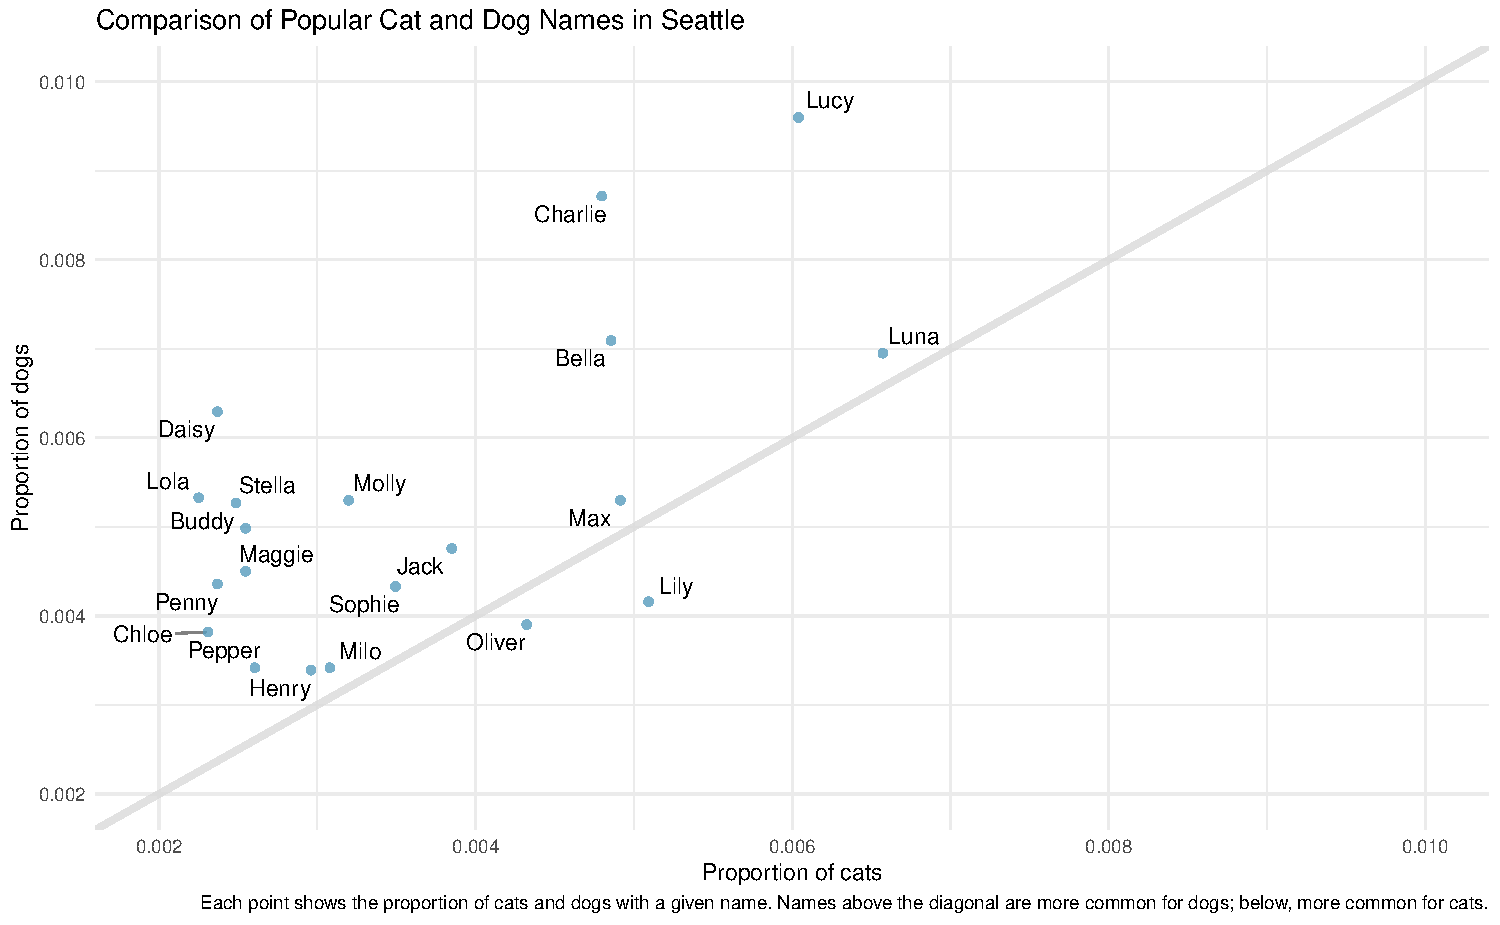
\includegraphics[width=0.8\linewidth]{hw-01-pet-names_files/figure-latex/popular_names-1}

\begin{enumerate}
\def\labelenumi{\arabic{enumi}.}
\tightlist
\item
  What names are more common for cats than dogs? The ones above the line
  or the ones below the line?

  \begin{itemize}
  \tightlist
  \item
    \textbf{Above the line} → proportion of dogs \textgreater{}
    proportion of cats (more common among dogs). \textbf{Names below the
    line} (e.g., \emph{lily}) are \textbf{more common for cats}. They
    have a higher proportion of cats with that name compared to dogs.
  \item
    \textbf{Below the line} → proportion of cats \textgreater{}
    proportion of dogs (more common among cats). \textbf{Names above the
    line} (e.g., \emph{daisy}) are \textbf{more common for dogs}. They
    have a higher proportion of dogs with that name compared to cats.
  \item
    The name \textbf{luna} is the most popular for both cats and dogs,
    with a proportion of approximately 0.055 for cats and 0.007 for
    dogs.
  \end{itemize}
\item
  Is the relationship between the two variables (proportion of cats with
  a given name and proportion of dogs with a given name) positive or
  negative? What does this mean in context of the data?

  \begin{itemize}
  \tightlist
  \item
    The relationship is \textbf{positive}: names that are common among
    cats tend also to be common among dogs. Names that are rare among
    cats tend also to be rare among dogs.
  \item
    In context, this means \textbf{popular names tend to be popular
    across both species}. For example, \emph{luna} and \emph{lucy} rank
    highly for both cats and dogs, while less popular names remain less
    common in both groups.
  \end{itemize}
\item
  Which name is the most popular for both cats and dogs?

  \begin{itemize}
  \tightlist
  \item
    The name \textbf{luna} is the most popular for both cats and dogs,
    with a proportion of approximately 0.055 for cats and 0.007 for
    dogs.
  \item
    The name \textbf{lucy} is also very popular for both species, with a
    proportion of approximately 0.006 for cats and 0.0097 for dogs.
  \end{itemize}
\end{enumerate}

The scatter plot above visualizes the relationship between the
popularity of names among cats and dogs in Seattle. Each point
represents a specific pet name, with its position determined by the
proportion of cats (x-axis) and dogs (y-axis) that bear that name. The
diagonal reference line indicates equal popularity between the two
species.

\textbf{Overall Name Distribution}

\begin{enumerate}
\def\labelenumi{\arabic{enumi}.}
\item
  \textbf{Diagonal Reference Line}: The diagonal line represents equal
  popularity between cats and dogs. Names falling exactly on this line
  would have the same proportional representation in both populations.
\item
  \textbf{Clustering Pattern}: Most names cluster in the lower left
  portion of the plot (between 0.002-0.006 on both axes), indicating
  that pet name distributions have a ``long tail'' - a few very popular
  names and many less common ones.
\end{enumerate}

\textbf{Species Preferences}

\begin{enumerate}
\def\labelenumi{\arabic{enumi}.}
\tightlist
\item
  \textbf{Dog-Preferred Names}: Names appearing above the diagonal line
  are proportionally more common for dogs:

  \begin{itemize}
  \tightlist
  \item
    ``Lucy'' shows the strongest dog preference (around 0.01 for dogs
    vs.~0.006 for cats)
  \item
    ``Charlie'' and ``Bella'' are also significantly more popular for
    dogs
  \item
    ``Daisy'' appears almost exclusively as a dog name
  \end{itemize}
\item
  \textbf{Cat-Preferred Names}: Names below the diagonal line are
  proportionally more common for cats:

  \begin{itemize}
  \tightlist
  \item
    ``Lily'' shows strong cat preference
  \item
    ``Oliver'', ``Sophie'', and ``Chloe'' are notably more popular among
    cats
  \item
    ``Pepper'' and ``Henry'' appear primarily as cat names
  \end{itemize}
\item
  \textbf{Similar Popularity Names}: Names near the diagonal have
  similar proportional popularity:

  \begin{itemize}
  \tightlist
  \item
    ``Luna'' is popular for both species but slightly more common for
    cats
  \item
    ``Max'' sits almost directly on the diagonal, indicating equal
    proportional popularity
  \end{itemize}
\end{enumerate}

\textbf{Statistical Insights}

\begin{enumerate}
\def\labelenumi{\arabic{enumi}.}
\item
  \textbf{Correlation Analysis}: The plot shows a positive correlation
  between cat and dog name preferences, suggesting that human naming
  tendencies transcend pet species. However, the correlation is
  moderate, not strong, indicating distinct species-specific
  preferences.
\item
  \textbf{Outliers}: ``Lucy'' and ``Charlie'' appear as statistical
  outliers in dog naming popularity, while ``Luna'' is an outlier for
  cats.
\item
  \textbf{Proportion Range}: Dog name proportions extend higher (up to
  0.01) than cat names (maximum around 0.008), suggesting slightly more
  naming concentration in dogs.
\end{enumerate}

\textbf{Cultural Implications}

This visualization reveals how pet naming conventions reflect human
cultural preferences while also showing species-specific patterns. The
differences may reflect perceptions of personality traits associated
with each species or gender associations with certain names. Names like
``Lucy'' may be perceived as fitting dog personalities, while ``Lily''
may be seen as more suitable for cat temperaments.

\begin{enumerate}
\def\labelenumi{\arabic{enumi}.}
\tightlist
\item
  \textbf{Shared Naming Trends}: The overlap in popular names indicates
  shared cultural influences in pet naming, with certain names being
  trendy across both species.
\item
  \textbf{Species-Specific Trends}: The distinct preferences for certain
  names reflect cultural perceptions of cats and dogs, with some names
  evoking traits associated with each species (e.g., ``Daisy'' for dogs,
  ``Lily'' for cats).
\item
  \textbf{Humanization of Pets}: The use of human names for pets
  reflects a broader cultural trend of anthropomorphizing animals,
  indicating the deep emotional bonds people form with their pets.
\end{enumerate}

🧶 ✅ ⬆️ \emph{Now is a good time to commit and push your changes to
GitHub with an appropriate commit message. Commit and push all changed
files so that your Git pane is cleared up afterwards. Make sure that
your last push to the repo comes before the deadline. You should confirm
that what you committed and pushed are indeed in your repo that we will
see by visiting your repo on GitHub.}

\end{document}
